\documentclass{standalone}
\usepackage{tikz}
\usetikzlibrary{patterns, positioning}
\usepackage[sfdefault]{ClearSans} %% option 'sfdefault' activates Clear Sans as the default text font
\usepackage[T1]{fontenc}

\begin{document}
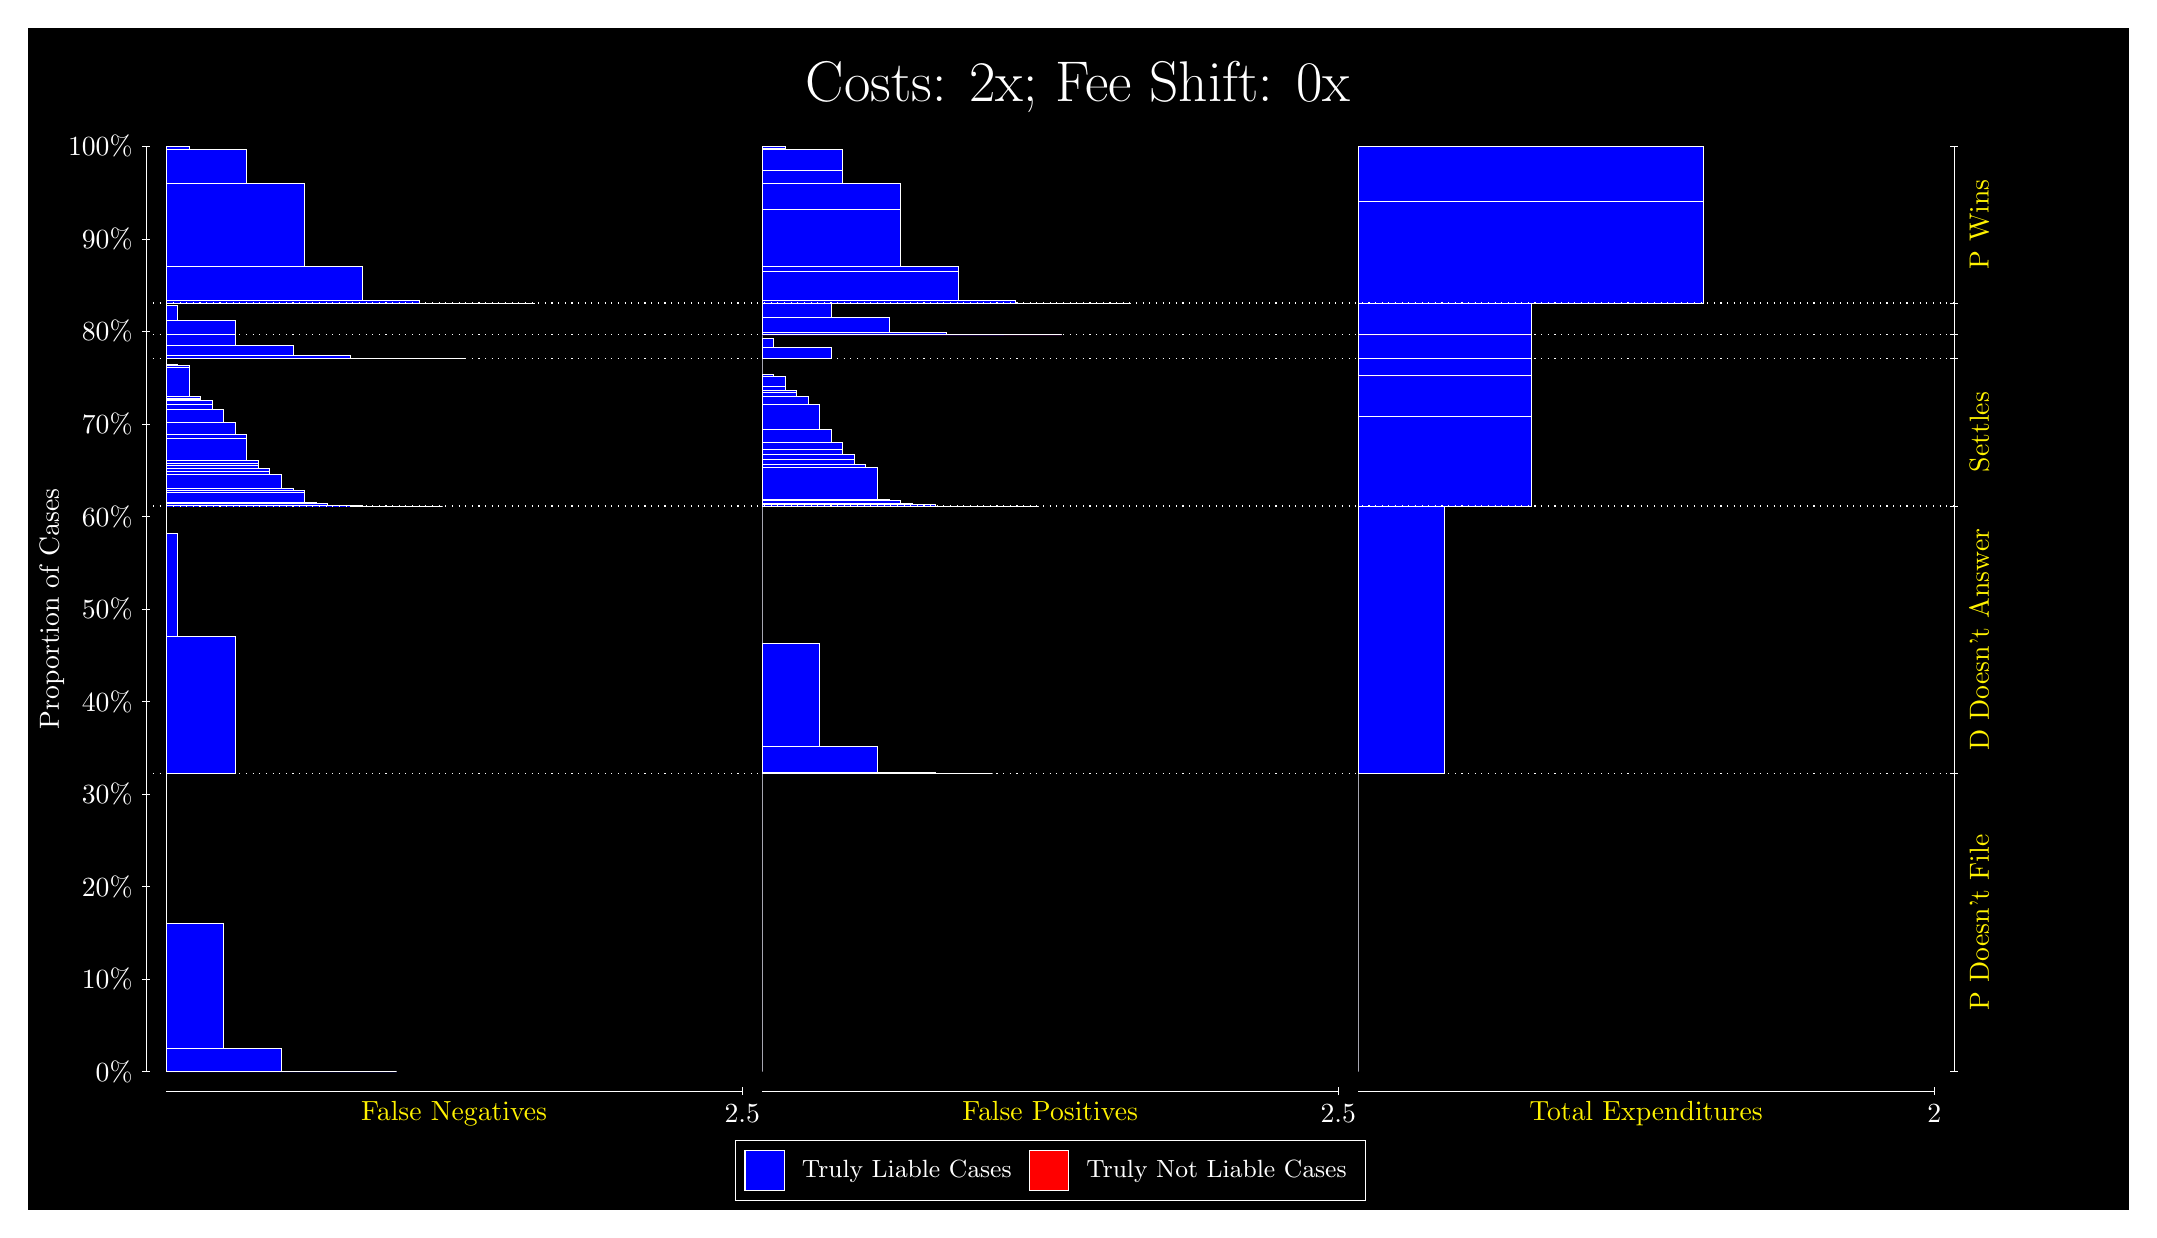
\begin{tikzpicture}
\draw[fill=black] (0,0) rectangle (26.667,15);
\draw[text=white] (0,13.5) rectangle (26.667,15) node[midway] {\huge Costs: 2x; Fee Shift: 0x};
\draw[white, very thin] (1.5,1.75) -- (1.5,13.5);
\node[rotate=90, text=white, anchor=center] at (0.3, 7.625) {Proportion of Cases};
\draw[white, very thin] (1.45,1.75) -- (1.55,1.75);
\node[text=white, anchor=east] at (1.45, 1.75) {0\%};
\draw[white, very thin] (1.45,2.925) -- (1.55,2.925);
\node[text=white, anchor=east] at (1.45, 2.925) {10\%};
\draw[white, very thin] (1.45,4.1) -- (1.55,4.1);
\node[text=white, anchor=east] at (1.45, 4.1) {20\%};
\draw[white, very thin] (1.45,5.275) -- (1.55,5.275);
\node[text=white, anchor=east] at (1.45, 5.275) {30\%};
\draw[white, very thin] (1.45,6.45) -- (1.55,6.45);
\node[text=white, anchor=east] at (1.45, 6.45) {40\%};
\draw[white, very thin] (1.45,7.625) -- (1.55,7.625);
\node[text=white, anchor=east] at (1.45, 7.625) {50\%};
\draw[white, very thin] (1.45,8.8) -- (1.55,8.8);
\node[text=white, anchor=east] at (1.45, 8.8) {60\%};
\draw[white, very thin] (1.45,9.975) -- (1.55,9.975);
\node[text=white, anchor=east] at (1.45, 9.975) {70\%};
\draw[white, very thin] (1.45,11.15) -- (1.55,11.15);
\node[text=white, anchor=east] at (1.45, 11.15) {80\%};
\draw[white, very thin] (1.45,12.325) -- (1.55,12.325);
\node[text=white, anchor=east] at (1.45, 12.325) {90\%};
\draw[white, very thin] (1.45,13.5) -- (1.55,13.5);
\node[text=white, anchor=east] at (1.45, 13.5) {100\%};

\draw[white, very thin] (24.457,1.75) -- (24.457,13.5);
\draw[white, very thin] (24.407,1.75) -- (24.507,1.75);
\node[anchor=west] at (24.407, 1.75) {};
\draw[white, very thin] (24.407,5.5358) -- (24.507,5.5358);
\node[anchor=west] at (24.407, 5.5358) {};
\draw[white, very thin] (24.407,8.9317) -- (24.507,8.9317);
\node[anchor=west] at (24.407, 8.9317) {};
\draw[white, very thin] (24.407,10.81) -- (24.507,10.81);
\node[anchor=west] at (24.407, 10.81) {};
\draw[white, very thin] (24.407,11.11) -- (24.507,11.11);
\node[anchor=west] at (24.407, 11.11) {};
\draw[white, very thin] (24.407,11.51) -- (24.507,11.51);
\node[anchor=west] at (24.407, 11.51) {};
\draw[white, very thin] (24.407,13.5) -- (24.507,13.5);
\node[anchor=west] at (24.407, 13.5) {};

\draw[white, very thin, fill=blue] (1.75,1.75) rectangle (4.6775,1.75);
\draw[white, very thin, fill=blue] (1.75,1.75) rectangle (3.9457,1.7525);
\draw[white, very thin, fill=blue] (1.75,1.7525) rectangle (3.2138,2.0502);
\draw[white, very thin, fill=blue] (1.75,2.0502) rectangle (2.4819,3.6338);
\draw[white, very thin, fill=red] (1.75,3.6338) rectangle (1.75,3.6338);
\draw[white, very thin, fill=blue] (1.75,3.6338) rectangle (1.75,5.5358);
\draw[white, very thin, fill=blue] (1.75,5.5358) rectangle (2.6283,7.2833);
\draw[white, very thin, fill=blue] (1.75,7.2833) rectangle (1.8964,8.5849);
\draw[white, very thin, fill=red] (1.75,8.5849) rectangle (1.75,8.5849);
\draw[white, very thin, fill=blue] (1.75,8.5849) rectangle (1.75,8.9317);
\draw[white, very thin, fill=blue] (1.75,8.9317) rectangle (5.2631,8.9317);
\draw[white, very thin, fill=blue] (1.75,8.9317) rectangle (4.9703,8.9318);
\draw[white, very thin, fill=blue] (1.75,8.9318) rectangle (4.6775,8.9318);
\draw[white, very thin, fill=blue] (1.75,8.9318) rectangle (4.5312,8.9333);
\draw[white, very thin, fill=blue] (1.75,8.9333) rectangle (4.3848,8.9333);
\draw[white, very thin, fill=blue] (1.75,8.9333) rectangle (4.3848,8.9333);
\draw[white, very thin, fill=blue] (1.75,8.9333) rectangle (4.2384,8.9352);
\draw[white, very thin, fill=blue] (1.75,8.9352) rectangle (4.092,8.9368);
\draw[white, very thin, fill=blue] (1.75,8.9368) rectangle (3.9457,8.9463);
\draw[white, very thin, fill=blue] (1.75,8.9463) rectangle (3.7993,8.9679);
\draw[white, very thin, fill=blue] (1.75,8.9679) rectangle (3.6529,8.9722);
\draw[white, very thin, fill=blue] (1.75,8.9722) rectangle (3.6529,8.9787);
\draw[white, very thin, fill=blue] (1.75,8.9787) rectangle (3.5065,9.1022);
\draw[white, very thin, fill=blue] (1.75,9.1022) rectangle (3.5065,9.1306);
\draw[white, very thin, fill=blue] (1.75,9.1306) rectangle (3.3602,9.1606);
\draw[white, very thin, fill=blue] (1.75,9.1606) rectangle (3.2138,9.3363);
\draw[white, very thin, fill=blue] (1.75,9.3363) rectangle (3.0674,9.37);
\draw[white, very thin, fill=blue] (1.75,9.37) rectangle (3.0674,9.4103);
\draw[white, very thin, fill=blue] (1.75,9.4103) rectangle (2.921,9.4474);
\draw[white, very thin, fill=blue] (1.75,9.4474) rectangle (2.921,9.4784);
\draw[white, very thin, fill=blue] (1.75,9.4784) rectangle (2.921,9.5168);
\draw[white, very thin, fill=blue] (1.75,9.5168) rectangle (2.7746,9.7969);
\draw[white, very thin, fill=blue] (1.75,9.7969) rectangle (2.7746,9.8372);
\draw[white, very thin, fill=blue] (1.75,9.8372) rectangle (2.6283,10.001);
\draw[white, very thin, fill=blue] (1.75,10.001) rectangle (2.4819,10.155);
\draw[white, very thin, fill=blue] (1.75,10.155) rectangle (2.3355,10.219);
\draw[white, very thin, fill=blue] (1.75,10.219) rectangle (2.3355,10.28);
\draw[white, very thin, fill=blue] (1.75,10.28) rectangle (2.1891,10.287);
\draw[white, very thin, fill=blue] (1.75,10.287) rectangle (2.1891,10.295);
\draw[white, very thin, fill=blue] (1.75,10.295) rectangle (2.1891,10.321);
\draw[white, very thin, fill=blue] (1.75,10.321) rectangle (2.0428,10.7);
\draw[white, very thin, fill=blue] (1.75,10.7) rectangle (2.0428,10.719);
\draw[white, very thin, fill=blue] (1.75,10.719) rectangle (1.8964,10.738);
\draw[white, very thin, fill=red] (1.75,10.738) rectangle (1.75,10.738);
\draw[white, very thin, fill=blue] (1.75,10.738) rectangle (1.75,10.81);
\draw[white, very thin, fill=blue] (1.75,10.81) rectangle (5.5558,10.81);
\draw[white, very thin, fill=blue] (1.75,10.81) rectangle (4.8239,10.812);
\draw[white, very thin, fill=blue] (1.75,10.812) rectangle (4.092,10.852);
\draw[white, very thin, fill=blue] (1.75,10.852) rectangle (3.3602,10.974);
\draw[white, very thin, fill=blue] (1.75,10.974) rectangle (2.6283,11.11);
\draw[white, very thin, fill=red] (1.75,11.11) rectangle (1.75,11.11);
\draw[white, very thin, fill=blue] (1.75,11.11) rectangle (2.6283,11.297);
\draw[white, very thin, fill=blue] (1.75,11.297) rectangle (1.8964,11.486);
\draw[white, very thin, fill=red] (1.75,11.486) rectangle (1.75,11.486);
\draw[white, very thin, fill=blue] (1.75,11.486) rectangle (1.75,11.51);
\draw[white, very thin, fill=blue] (1.75,11.51) rectangle (6.4341,11.51);
\draw[white, very thin, fill=blue] (1.75,11.51) rectangle (5.7022,11.51);
\draw[white, very thin, fill=blue] (1.75,11.51) rectangle (4.9703,11.543);
\draw[white, very thin, fill=blue] (1.75,11.543) rectangle (4.2384,11.974);
\draw[white, very thin, fill=blue] (1.75,11.974) rectangle (3.5065,13.035);
\draw[white, very thin, fill=blue] (1.75,13.035) rectangle (2.7746,13.467);
\draw[white, very thin, fill=blue] (1.75,13.467) rectangle (2.0428,13.5);
\draw[white, very thin, fill=red] (1.75,13.5) rectangle (1.75,13.5);
\draw[white, very thin, fill=blue] (1.75,13.5) rectangle (1.75,13.5);
\draw[white, very thin, fill=red] (9.3189,1.75) rectangle (9.3189,1.75);
\draw[white, very thin, fill=blue] (9.3189,1.75) rectangle (9.3189,5.5358);
\draw[white, very thin, fill=red] (9.3189,5.5358) rectangle (12.246,5.5358);
\draw[white, very thin, fill=blue] (9.3189,5.5358) rectangle (12.246,5.5358);
\draw[white, very thin, fill=blue] (9.3189,5.5358) rectangle (11.515,5.5481);
\draw[white, very thin, fill=blue] (9.3189,5.5481) rectangle (10.783,5.8826);
\draw[white, very thin, fill=blue] (9.3189,5.8826) rectangle (10.051,7.1842);
\draw[white, very thin, fill=blue] (9.3189,7.1842) rectangle (9.3189,8.9317);
\draw[white, very thin, fill=red] (9.3189,8.9317) rectangle (12.832,8.9317);
\draw[white, very thin, fill=blue] (9.3189,8.9317) rectangle (12.832,8.9317);
\draw[white, very thin, fill=red] (9.3189,8.9317) rectangle (12.539,8.9317);
\draw[white, very thin, fill=blue] (9.3189,8.9317) rectangle (12.539,8.9317);
\draw[white, very thin, fill=red] (9.3189,8.9317) rectangle (12.246,8.9317);
\draw[white, very thin, fill=blue] (9.3189,8.9317) rectangle (12.246,8.9318);
\draw[white, very thin, fill=blue] (9.3189,8.9318) rectangle (12.1,8.9318);
\draw[white, very thin, fill=red] (9.3189,8.9318) rectangle (11.954,8.9318);
\draw[white, very thin, fill=blue] (9.3189,8.9318) rectangle (11.954,8.9319);
\draw[white, very thin, fill=blue] (9.3189,8.9319) rectangle (11.807,8.9319);
\draw[white, very thin, fill=red] (9.3189,8.9319) rectangle (11.661,8.9319);
\draw[white, very thin, fill=blue] (9.3189,8.9319) rectangle (11.661,8.9326);
\draw[white, very thin, fill=blue] (9.3189,8.9326) rectangle (11.515,8.9521);
\draw[white, very thin, fill=red] (9.3189,8.9521) rectangle (11.368,8.9521);
\draw[white, very thin, fill=blue] (9.3189,8.9521) rectangle (11.368,8.9547);
\draw[white, very thin, fill=blue] (9.3189,8.9547) rectangle (11.222,8.9625);
\draw[white, very thin, fill=blue] (9.3189,8.9625) rectangle (11.075,8.9719);
\draw[white, very thin, fill=red] (9.3189,8.9719) rectangle (11.075,8.9719);
\draw[white, very thin, fill=blue] (9.3189,8.9719) rectangle (11.075,9.003);
\draw[white, very thin, fill=blue] (9.3189,9.003) rectangle (10.929,9.0221);
\draw[white, very thin, fill=red] (9.3189,9.0221) rectangle (10.783,9.0221);
\draw[white, very thin, fill=blue] (9.3189,9.0221) rectangle (10.783,9.42);
\draw[white, very thin, fill=blue] (9.3189,9.42) rectangle (10.636,9.4616);
\draw[white, very thin, fill=red] (9.3189,9.4616) rectangle (10.49,9.4616);
\draw[white, very thin, fill=blue] (9.3189,9.4616) rectangle (10.49,9.5224);
\draw[white, very thin, fill=blue] (9.3189,9.5224) rectangle (10.49,9.5867);
\draw[white, very thin, fill=blue] (9.3189,9.5867) rectangle (10.344,9.6464);
\draw[white, very thin, fill=blue] (9.3189,9.6464) rectangle (10.344,9.7406);
\draw[white, very thin, fill=blue] (9.3189,9.7406) rectangle (10.197,9.9043);
\draw[white, very thin, fill=blue] (9.3189,9.9043) rectangle (10.051,10.225);
\draw[white, very thin, fill=blue] (9.3189,10.225) rectangle (9.9044,10.331);
\draw[white, very thin, fill=blue] (9.3189,10.331) rectangle (9.758,10.372);
\draw[white, very thin, fill=blue] (9.3189,10.372) rectangle (9.758,10.405);
\draw[white, very thin, fill=blue] (9.3189,10.405) rectangle (9.6116,10.458);
\draw[white, very thin, fill=blue] (9.3189,10.458) rectangle (9.6116,10.581);
\draw[white, very thin, fill=blue] (9.3189,10.581) rectangle (9.4652,10.611);
\draw[white, very thin, fill=blue] (9.3189,10.611) rectangle (9.3189,10.81);
\draw[white, very thin, fill=red] (9.3189,10.81) rectangle (10.197,10.81);
\draw[white, very thin, fill=blue] (9.3189,10.81) rectangle (10.197,10.946);
\draw[white, very thin, fill=blue] (9.3189,10.946) rectangle (9.4652,11.068);
\draw[white, very thin, fill=blue] (9.3189,11.068) rectangle (9.3189,11.11);
\draw[white, very thin, fill=red] (9.3189,11.11) rectangle (13.125,11.11);
\draw[white, very thin, fill=blue] (9.3189,11.11) rectangle (13.125,11.11);
\draw[white, very thin, fill=blue] (9.3189,11.11) rectangle (12.393,11.11);
\draw[white, very thin, fill=blue] (9.3189,11.11) rectangle (11.661,11.134);
\draw[white, very thin, fill=blue] (9.3189,11.134) rectangle (10.929,11.323);
\draw[white, very thin, fill=blue] (9.3189,11.323) rectangle (10.197,11.51);
\draw[white, very thin, fill=red] (9.3189,11.51) rectangle (14.003,11.51);
\draw[white, very thin, fill=blue] (9.3189,11.51) rectangle (14.003,11.51);
\draw[white, very thin, fill=red] (9.3189,11.51) rectangle (13.271,11.51);
\draw[white, very thin, fill=blue] (9.3189,11.51) rectangle (13.271,11.51);
\draw[white, very thin, fill=red] (9.3189,11.51) rectangle (12.539,11.51);
\draw[white, very thin, fill=blue] (9.3189,11.51) rectangle (12.539,11.543);
\draw[white, very thin, fill=blue] (9.3189,11.543) rectangle (11.807,11.914);
\draw[white, very thin, fill=red] (9.3189,11.914) rectangle (11.807,11.914);
\draw[white, very thin, fill=blue] (9.3189,11.914) rectangle (11.807,11.975);
\draw[white, very thin, fill=blue] (9.3189,11.975) rectangle (11.075,12.703);
\draw[white, very thin, fill=red] (9.3189,12.703) rectangle (11.075,12.703);
\draw[white, very thin, fill=blue] (9.3189,12.703) rectangle (11.075,13.036);
\draw[white, very thin, fill=blue] (9.3189,13.036) rectangle (10.344,13.19);
\draw[white, very thin, fill=blue] (9.3189,13.19) rectangle (10.344,13.467);
\draw[white, very thin, fill=blue] (9.3189,13.467) rectangle (9.6116,13.473);
\draw[white, very thin, fill=blue] (9.3189,13.473) rectangle (9.6116,13.5);
\draw[white, very thin, fill=blue] (9.3189,13.5) rectangle (9.3189,13.5);
\draw[white, very thin, fill=red] (16.888,1.75) rectangle (16.888,1.75);
\draw[white, very thin, fill=blue] (16.888,1.75) rectangle (16.888,5.5358);
\draw[white, very thin, fill=red] (16.888,5.5358) rectangle (17.986,5.5358);
\draw[white, very thin, fill=blue] (16.888,5.5358) rectangle (17.986,8.9317);
\draw[white, very thin, fill=red] (16.888,8.9317) rectangle (19.083,8.9317);
\draw[white, very thin, fill=blue] (16.888,8.9317) rectangle (19.083,10.071);
\draw[white, very thin, fill=red] (16.888,10.071) rectangle (19.083,10.071);
\draw[white, very thin, fill=blue] (16.888,10.071) rectangle (19.083,10.587);
\draw[white, very thin, fill=red] (16.888,10.587) rectangle (19.083,10.587);
\draw[white, very thin, fill=blue] (16.888,10.587) rectangle (19.083,10.81);
\draw[white, very thin, fill=red] (16.888,10.81) rectangle (19.083,10.81);
\draw[white, very thin, fill=blue] (16.888,10.81) rectangle (19.083,11.11);
\draw[white, very thin, fill=red] (16.888,11.11) rectangle (19.083,11.11);
\draw[white, very thin, fill=blue] (16.888,11.11) rectangle (19.083,11.51);
\draw[white, very thin, fill=red] (16.888,11.51) rectangle (21.279,11.51);
\draw[white, very thin, fill=blue] (16.888,11.51) rectangle (21.279,12.802);
\draw[white, very thin, fill=red] (16.888,12.802) rectangle (21.279,12.802);
\draw[white, very thin, fill=blue] (16.888,12.802) rectangle (21.279,13.5);
\draw[white, dotted] (1.5,5.5358) -- (24.457,5.5358);
\draw[white, dotted] (1.5,8.9317) -- (24.457,8.9317);
\draw[white, dotted] (1.5,10.81) -- (24.457,10.81);
\draw[white, dotted] (1.5,11.11) -- (24.457,11.11);
\draw[white, dotted] (1.5,11.51) -- (24.457,11.51);
\draw[white, very thin] (1.75,1.5) -- (9.0689,1.5);
\node[text=yellow, anchor=north] at (5.4094, 1.5) {False Negatives};
\draw[white, very thin] (9.0689,1.45) -- (9.0689,1.55);
\node[text=white, anchor=north] at (9.0689, 1.45) {2.5};

\draw[white, very thin] (9.3189,1.5) -- (16.638,1.5);
\node[text=yellow, anchor=north] at (12.978, 1.5) {False Positives};
\draw[white, very thin] (16.638,1.45) -- (16.638,1.55);
\node[text=white, anchor=north] at (16.638, 1.45) {2.5};

\draw[white, very thin] (16.888,1.5) -- (24.207,1.5);
\node[text=yellow, anchor=north] at (20.547, 1.5) {Total Expenditures};
\draw[white, very thin] (24.207,1.45) -- (24.207,1.55);
\node[text=white, anchor=north] at (24.207, 1.45) {2};

\node[text=yellow, centered, rotate=90] at (24.777, 3.6429) {P Doesn't File};
\node[text=yellow, centered, rotate=90] at (24.777, 7.2337) {D Doesn't Answer};
\node[text=yellow, centered, rotate=90] at (24.777, 9.8707) {Settles};


\node[text=yellow, centered, rotate=90] at (24.777, 12.505) {P Wins};

\draw (12.978300999999998,1.5) node[draw=none] (baseCoordinate) {};
\begin{scope}[align=center]
        \matrix[scale=0.5, draw=white, below=0.5cm of baseCoordinate, nodes={draw}, column sep=0.1cm]{
            \node[rectangle, draw, minimum width=0.5cm, minimum height=0.5cm, fill=blue] {}; &
            \node[draw=none, font=\small, text=white] (B) {Truly Liable Cases}; &
            \node[rectangle, draw, minimum width=0.5cm, minimum height=0.5cm, fill=red] {}; &
            \node[draw=none, font=\small, text=white] (B) {Truly Not Liable Cases}; \\
            };
\end{scope}

\end{tikzpicture}
\end{document}